% 26-06-00 start collecting notes for this chapter
% 28-06-00 in shape

\chapter{Linkage tests for small pedigrees}

\section{Introduction}

Linkage analysis of complex traits is commonly performed using parametric lod
score method and nonparametric allele-sharing method.  Parametric tests
generalise the traditional lod score method by maximising over recombination
parameters while treating allele frequencies and mode of inheritance as
nuisance parameters (Risch 1984; Clerget-Darpoux et al.  1986; Elston 1994;
Hodge \& Elston 1994).  The MOD score is defined as the maximum lod score over
mode of inheritance.  Minor misspecification of mode of inheritance can affect
estimation of recombination parameters but not seriously reduce lod score
(Clerget-Darpoux et al.  1986).  However, it has the undesirable property that
its distribution is unknown under the null hypothesis, with penetrance playing
a role in the alternative hypothesis but not defined under the null.  Curtis \&
Sham (1995a) attempted to amend this by introducing MFLOD (model-free lod
score), obtained via the computer program MFLINK, where maximised lod score and
maximised admixture lod score were also calculated.  Interestingly both were
observed approximately proportional to $\chi^2$ statistics and occasionally
larger than MFLOD.  Lin et al.  (1997) therefore named them as MLOD (lod score
maximised over disease models) and MALOD (admixture lod score maximised over
disease models).  Nonparametric allele-sharing statistics are mostly
generalisation of sib-pair statistics (Suarez et al.  1978, Blackwelder \&
Elston 1985) by using IBS (Weeks \& Lange 1988) and IBD information among all
affected relative pairs (Whittemore \& Halpern 1994a, 1994b; Kruglyak et al.
1996).

The performance of these statistics depends on family structure, number of
affected individuals, mode of inheritance, location and informativeness of
markers (e.g., Boehnke 1991; Ott 1992; Terwilliger \& Ott 1994).  In addition
to mode of inheritance and recombination rate between markers and the disease
genes, power of allele-sharing methods also depends on how allele-sharing
within a pedigree is scored and how these scores are weighted across pedigrees.
These have generated considerable interests (Durner et al.  1992; Risch \&
Zhang 1995; Davis et al.  1996; Sham et al.  1997; Davis \& Weeks 1997; Hodge
1997; Hodge 1998; Goldin, Greenberg et al.  1998; Durner et al.  1999; McPeek
1999; Blackwelder \& Elston 1985; Risch 1990a,b,c; Holmans 1993; Kruglyak \&
Lander 1995; Hauser et al.  1996; Whittemore 1996; Kruglyak et al.  1996; Kong
\& Cox 1997; Hauser \& Boehnke 1998; McCarthy et al.  1998; Abreu et al.  1999;
Teng \& Siegmund 1998; Dudoit \& Speed 2000; Dupuis \& van Eerdewegh 2000;
Liang et al.  2001; Shih \& Whittemore 2001).  Unfortunately, Sengul et al.
(2001) noted that it is hard to make direct comparison of these investigations,
owing to differences in these study designs.

Lin et al.  (1997) used computer simulation and simple family types to evaluate
the performance of parametric and NPL statistics under single gene models with
linkage homogeneity and heterogeneity and concluded that, under a model with a
major gene effect, likelihood-based methods tend to be more powerful.  For a
minor gene effect, the NPL statistics were generally superior to the other
tests.

\subsection*{Chapter aims}

This chapter concerns the comparison of power of parametric and nonparametric
linkage tests under complete marker information.  The parametric and
non-parametric linkage test statistics include MLOD, MALOD, MFLOD, and NPLs.
Four types of simple pedigrees and their mixture and several modes of
inheritance are used to examine behaviour of these statistics under both
linkage homogeneity and heterogeneity.  In contrast to Lin et al.  (1997), the
power comparisons will be based on exact calculations.


\section{Methods}

\subsection*{Definition of test statistics}

We restrict ourselves to the usual generalised single locus model, in
which the disease locus is biallelic consisting of both a disease allele
and a normal allele. Note there are other single locus models, for
instance those with multiple alleles (Nielsen, Ehm \& Weir 1998; Nielsen
\& Weir 1999, 2001). We also allow for mixture of families exist in the
study sample, in which linkage only occurs in a subset of families. We
study several two-point linkage statistics under these assumptions.

Let $q$ = the frequency of the disease allele; $f_i$ = the penetrances,
namely the conditional probabilities of the disease given $i$ copies of
the disease allele, $i=0, 1, 2$; $\theta$ = the recombination fraction
between the disease locus and the marker locus; $\alpha$ = the proportion
of families with linkage. The lod score and admixture lod score under this
disease model are denoted as {\bf LOD} and {\bf ALOD}, respectively.  To
calculate MLOD, MALOD and MFLOD, disease model parameters are constrained
to produce the correct population disease prevalence ($K$),
\begin{eqnarray}
f_0 = f_1, f_2 = 1-f_1(1-K)/K  &\mbox{when}& f_1\leq K \cr
f_2 = f_1, f_0 = (1-f_1)K/(1-K)  &\mbox{when}& f_1>K\label{f1}
\end{eqnarray}
which implies that only $f_1$ is free, and that and $q$ is given by
solving $q^2f_2+2q(1-q)f_1+(1-q)^2f_0 = K$ (Curtis \& Sham, 1995).  
Specifically, $f_1$ is restricted to vary along the sides of the triangle
of $(0,0,1)$, $(K,K,K)$ and $(0, 1, 1)$, so that all the parameters are
well characterised by $f_1$ and $K$.  By using marker data (M) and disease
phenotype ($D$), MLOD, MALOD and MFLOD can be evaluated as a function of
$f_1$ and $\alpha$ at a test position $\theta=t$, as follows (Sham, Lin et
al.  2000).

{\bf MLOD}:  the maximum lod score obtained over all feasible transmission
models, i.e. for a given value of $\theta=t$,
\begin{eqnarray*}
~ &~&\max\limits_{f_1}
\log_{10}(P(D,M;\theta=t,f_1)/P(D,M;\theta=0.5,f_1)) \cr
&=&\max\limits_{f_1}\log_{10}(P(M|D;\theta=t,f_1)/P(M)) \cr
&=&\max\limits_{f_1}\log_{10}(P(M|D;\theta=t,f_1)/P(M|D;\theta=t;f_1=K))
\end{eqnarray*}
with $\alpha$ being fixed to be 1.  For instance, the second step holds since
under no linkage (i.e., $\theta=0.5$) the disease locus and the marker are
independent.  The only free parameter associated with MLOD is $f_1$, which is
allowed to vary between 0 and 1, with the null hypothesis value being $f_1=K$.
MLOD is therefore the logarithm of ratio of the likelihoods of two nested
models, and $(2\ln 10)$MLOD is asymptotically distributed as $\chi_1^2$
(2-sided, since $f_1$ can be greater or less than $K$).

{\bf MALOD}:  the maximum admixture lod score (maximum over these transmission
models and $\alpha$), i.e,
\begin{eqnarray*}
~&~&\max\limits_{\alpha,f_1} \log_{10}(P(D,M;\theta=t,\alpha,f_1)/P(D,M;\theta=0.5,
~\mbox{or}~ \alpha=0,f_1))\cr
&=&\max\limits_{\alpha,f_1} \log_{10}(P(M|D;\theta=t,\alpha,f_1)/P(M))\cr
&=&\max\limits_{\alpha,f_1} \log_{10}(P(M|D;\theta=t; \alpha, f_1)/P(M|D;
\theta = t, \alpha=0 ~\mbox{or}~f_1=K))
\end{eqnarray*}
MALOD statistic is characterised by two free parameters, $f_1$ and $\alpha$,
which are fixed and completely confounded under the null hypothesis (which can
be specified by either $f_1=K$ or $\alpha=0$), therefore $(2\ln 10)$MALOD is
somewhat conservative for an asymptotic distribution of a $50:50$ mixture of
$\chi_0^2$ and $\chi_2^2$, under the null hypothesis that linkage is absent,
and that it would be more unfavourable to refer MALOD to $\chi^2$ distribution
with two degrees of freedom and would yield a conservative test.

{\bf MFLOD}:  the lod score obtained from the difference between likelihood
maximising over $f_1$, $\alpha$ and likelihood maximising $f_1$ but setting
$\alpha$ to be zero, i.e.,
\begin{eqnarray*}
\max\limits_{\alpha,f_1}
\log_{10}(P(D,M|\alpha,\theta=t,f_1)/\max\limits_{f_1}P(D,M|\alpha=0,\theta=0,f_1))
\end{eqnarray*}
Asymptotically, $(2\ln10)$MFLOD is $\chi^2$ with one degree of freedom as the
only parameter (free in the numerator likelihood but fixed to 0 in the
denominator likelihood) is $\alpha$, which differs from MLOD and MALOD in that
it is the logarithm of a ratio of the joint likelihoods of marker and disease
phenotypes, rather than the logarithm of a ratio of the conditional likelihoods
of marker phenotypes given disease phenotypes.

{\bf NPL statistics}:  which include NPLpair and NPLall and are based on normal
approximations of score functions $S_{pair}$ and $S_{all}$.  Let $n_A$ be the
number of affected relatives in a pedigree, $h$ a collection of alleles
generated by taking one allele from each affected individuals (there are
$2^{n_A}$ possible collections), $2f$ the total number of founder alleles
(total number of IBD alleles) in the pedigree, $b(h)$ the total number of
appearances of a founder allele in the collection $h$, the two score functions
assign numerical values to all possile IBD configurations,
\begin{eqnarray*}
S_{pair} &=&{2}/{[n_A(n_A-1)]}\sum_{1\leq k\leq l\leq n_A}
\left[\frac{1}{4}\sum_{a=1}^2\sum_{b=1}^2\delta(s_{ka},s_{lb})\right]
\end{eqnarray*} and
\begin{eqnarray*}
S_{all}&=&2^{-n_A}\sum_h \left[\Pi_{i=1}^{2f}b_i(h)!\right]
\end{eqnarray*}
where $\delta(.,.)$ is the Kronecker delta function with $\delta(s,s')=1$ or
$0$ according to whether or not alleles $s$ and $s'$ are IBD, and $(s_{11},
s_{12},\ldots,s_{n1},s_{n2})$ is the inheritance vector indicating which of the
$2f$ founder alleles the nonfounders inherit.  With score function $S_i$ thus
defined, NPL is then obtained as $Z=\sum_{i=1}^mZ_i/\sqrt{m}$,
$Z_i=(S_i-\mu_i)/\sigma_i$, with $m$ being number of pedigrees in the sample,
$\mu_i$ and $\sigma_i$ being the null mean and null standard deviation of
$S_i$.  In words, NPLpair is based on number of pairs of alleles from distinct
pedigree members are IBD.  NPLall is based on the average number of
permutations that preserve a collection $h$ (Kruglyak et al.  1996; Sham 1998;
Shih \& Whittemore 2001).

\subsection*{Genetic models}

Four models of major genes with minor effects are considered (see
Table~\ref{models2}).  For each model, the table gives the penetrance ($f_i$),
prevalence ($K$), and the conditional probabilities ($c_i$) of having $i$
copies, $i=0, 1, 2$, of the disease alleles among affected individuals.  Two
of the models have high penetrance genes.  These are common recessive (CR) and
common dominant (CD).  The use of common recessive and dominant models
conforms to the notion that in linkage analysis of complex traits it is
preferable to consider both dominant and recessive models (Clerget-Darpoux et
al.  1986; Hodge et al.  1997).  The other two models are multiplicative (MM1
and MM2) with genotypic relative risks 4 and 3, respectively. The first 
model, MM1, has been used in Sham \& Curtis (1995a); it also gives the same 
prevalence as MM2. 

\begin{table}[h]
\centering
\caption{The four genetic models\label{models2}}
\begin{tabular}{lcccccccc}
\\
\hline
Model             & $f_2$ & $f_1$ & $f_0$ & $q$ & $K$ & $c_2$ & $c_1$ & $c_0$\\
\hline
\\
Common recessive (CR) & .50 &  .005 & .005 & .100 & .01 &  .503 & .090 & .407\\
Common dominant (CD) & .50 &  .500 & .005 & .005 & .01 &  .001 & .501 & .498\\
Multiplicative model 1 (MM1) &   .80 &  .200 & .050 & .130 & .10 &  .140 & .468 & .392\\
Multiplicative model 2 (MM2) &   .45 &  .150 & .050 & .207 & .10 &  .193 & .493 & .315\\
\hline
\end{tabular}
\end{table}

\subsection*{Pedigree configurations and marker information}

Four typical family types (Figure~\ref{f4}) and their mixture are examined.
This allows for factors such as number of affected/unaffected individuals in a
family and the availability of distant relatives to be examined.  Families 1-3
are nuclear families, each containing an affected sib pair, with an extra
affected sib in family 2 and an extra unaffected sib in family 3.  Family 4 is
extended to have a affected cousin with an unaffected sib, the trait phenotypes
of unaffected individuals in this family are assumed to be unknown.  The
proportions of four families in the family mixture are 0.5, 0.2, 0.2, 0.1,
respectively.

To control for effect of allele frequencies, a fully informative marker is
assumed.  To focus on comparison of test statistics, the recombination rate
($\theta$) is assumed to be 0.  Marker phenotypes are assumed to be available
to all members of the families.  There are 4, 16, 16, and 256 possible marker
genotype configurations ($n$, shortened for genotype configurations below) for
family types 1-4.

\subsection*{Method of computing asymptotic distributions}

Under no linkage, each genotype configuration occurs with equal probability
$(1/n)$, compared to $p_i^1$ under linkage and $(p_i^1+1/n)/2$ under admixture
of $\alpha$=0.5, $i=1, \ldots, n$.  These probabilities are used to calculate
the expected values of the log-likelihoods, LOD scores and ALOD scores, over
fine grid values of $f_1$ and $\alpha$.  Appropriate values maximised over
these grids provide estimate of noncentrality parameter estimates per pedigree
for MLOD ($f_1$), MALOD ($f_1$ and $\alpha$) and MFLOD (difference between
log-likelihoods maximised over $f_1$, $\alpha$ and over $f_1$).  The means and
standard deviations of all statistics over all possible genotype configurations
are calculated under the null hypothesis of no linkage and under alternatives
of linkage and linkage heterogeneity.

\begin{figure}[h]
\centering
\epsfig{figure=f4.ps,width=6.2in,height=2.5in}
%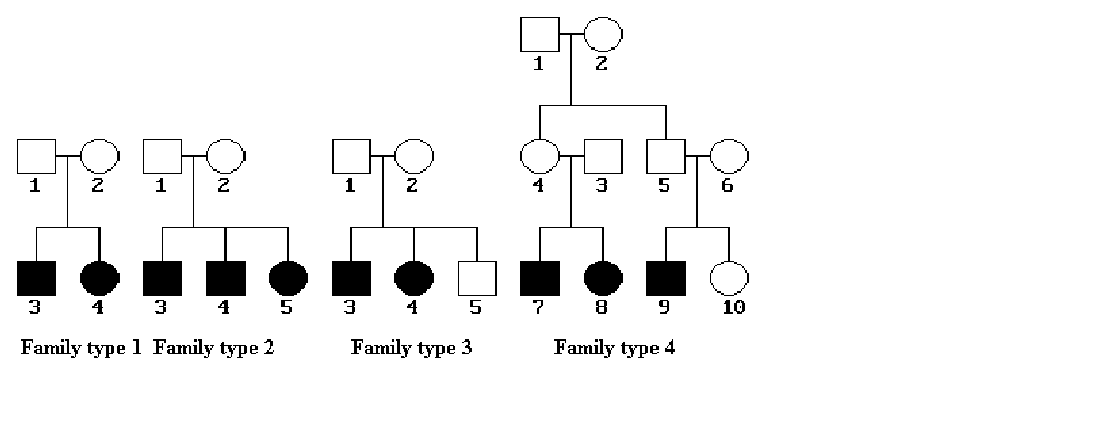
\includegraphics[width=6.2in,height=2.5in]{f4.bmp}
\caption{The four family types\label{f4}}
\end{figure}

For a normally distributed test statistic with mean 0 and variance 1 under the
null hypothesis and mean $m$ and variance $v$ under the alternative, the sample
size required based on 1-sided normal approximation for type I and type II
error rates $\alpha=0.0001$ and $\beta=0.1$ is $N=\lceil {[(3.719+1.282
\sqrt{v})}/{m}]^2\rceil$, where the ceiling function $\lceil.\rceil$ always
rounds fractional argument up by 1.  This has been used for NPL, so has been
for LOD and ALOD, as they are calculated directly without maximisation while
Central Limit Theorem would justify its use given large number of families.
For MLOD, MALOD and MFLOD the required sample sizes are calculated according to
their noncentrality parameters per pedigree.  The required sample sizes are
obtained for type I error rates $\alpha$=0.0001, 0.00001 and 90\% power.  The
noncentrality parameters for $\chi^2$ distribution with degrees of freedom of 1
and 2 are 26.76 and 29.92 for 2-sided tests (25.00 and 28.11 for 1-sided).

%The corresponding deviates are 3.09, 3.72 for normal, 10.83, 15.14 for $\chi^2$
%with degree of freedom 1 and 13.82, 18.42 for $\chi^2$ with degrees of freedom
%2.

The mean and variance of a statistic for family mixture can be obtained from
means and variances of individual families over all genotype configurations, as
$\sum_{j=1}^4 \tau_j m_j$ and $\sum_{j=1}^4 \tau_j (v_j+m_j^2) - (\sum_{j=1}^4
\tau_j m_j)^2$, where $\tau$ is the proportion of family type $j$ in the
mixture, and $m_j$ and $v_j$ are the mean and variance of a statistic for
family type $j$, respectively.

\subsection*{Simulation studies}

Empirical distributions for these statistics under the null hypothesis were
obtained via computer simulation.  Replicates are obtained from multinomial
distributions of genotype configurations given different family types and
transmission models under the null hypothesis.  The numbers of replicates are
determined by LOD and ALOD such that according to asymptotic theory, a
LOD score or a ALOD score test should have 90\% power at significance 0.0001.
Test statistics are calculated for 10,000 simulated samples in order to provide
their empirical distributions.  These distributions are compared with the
normal or $\chi^2$ distributions at the critical value for a significance
level of 0.001, to see if the tests produce correct p values.

%As an example, the means and variances for model 1 and family mixture under the
%null are -0.353, 0.281 for LOD and -0.074, 0.051 for ALOD, after
%standardisation they become 1.287, 0.908 for LOD and 0.720, 1.738 for ALOD, the
%required sample sizes for LOD and ALOD are 15 and 57, respectively.  Thresholds
%used in simulation for LOD and ALOD are thus $3.0 \sqrt{15 \times 0.281} + 15
%\times (-0.353)=0.864$ and $ 3.0 \sqrt{57 \times 0.051} + 57 \times
%(-0.074)=0.896$.

We shall illustrate the calculations with family 1, which has four possible
genotype configurations.  If the parental genotypes are (12, 34) and the first
offspring is assigned genotype 13, then the four configurations are specified
by the second offspring (13, 14, 23, 24).  We denote these configurations are
denoted as $i=1,\ldots,4$, so that the following quantities can be obtained,

$l_i$ - likelihood of linkage under a true model

$u_i$ - likelihood of no linkage

$p_i^0$ - probability of genotype configuration under no linkage

$p_i^\alpha$ - probability of genotype configuration under admixture

$p_i^1$ - probability of genotype configuration under full linkage

$lod_i$ - lod score for a given genotype configuration

$alod_i$ - admixture lod score for a given genotype configuration

\noindent
We use {\bf VITESSE} (O'Connell \& Weeks 1995; O'Connell 2001) to obtain the
quantities $\log_{10}(l_i)$ and $\log_{10}(u_i)$. Then
\begin{eqnarray*}
p_i^0 &=& 1/4 \cr
p_i^1 &=& l_i/\sum_{j=1}^4l_j=10^{\log_{10}(l_i)+M}/\sum_{j=1}^410^{\log_{10}(l_j)+M},\quad i=1, \ldots, n\cr
p_i^\alpha &=& (1-\alpha)p_k^0+\alpha p_k^1
\end{eqnarray*}
where $M$ is a large number used to avoid underflow. As usual,
$lod_i=\log_{10}(l_i/u_i)$, $alod_i=\log_{10}((\alpha
l_i+(1-\alpha)u_i)/u_i)=\log_{10}(\alpha 10^{lod_i}+(1-\alpha))$.
Further we have under no linkage
\begin{eqnarray*}
\mbox{E(LOD)}  &=& \sum_{j=1}^4p_j^0lod_j\cr
\mbox{V(LOD)}  &=& \sum_{j=1}^4p_j^0lod_j^2-[\mbox{E(LOD)}]^2\cr
\mbox{E(ALOD)} &=& \sum_{j=1}^4p_j^0alod_j \cr
\mbox{V(ALOD)} &=& \sum_{j=1}^4p_j^0alod_j^2-[\mbox{E(ALOD)}]^2
\end{eqnarray*}
and under linkage
\begin{eqnarray*}
\mbox{E(LOD)}  &=& \sum_{j=1}^4p_j^1lod_i \cr
\mbox{V(LOD)}  &=& \sum_{j=1}^4p_j^1lod_j^2-[\mbox{E(LOD)}]^2 \cr
\mbox{E(ALOD)} &=& \sum_{j=1}^4p_j^\alpha alod_j \cr
\mbox{V(ALOD)} &=& \sum_{j=1}^4p_j^\alpha alod_j^2-[\mbox{E(ALOD)}]^2
\end{eqnarray*}

Using these quantitities the required sample size at significance level of
0.0001 and 90\% power can be calculated for LOD and ALOD, which will be
used in setting their thresholds in simulations under the null hypothesis
and for calculation of MLOD, MALOD and MFLOD.  Note that under the null
hypothesis means and variances of LOD and ALOD may deviate slightly from 0
and 1, the calculation of sample sizes takes into account of this fact by
appropriate standardisation according to their means and variances under
the null.  Also note that calculations for LOD and ALOD are carried out
under true models of linkage and no linkage and we assume $\alpha=0.5$.  
The calculations of NPLpair and NPLall are similar to LOD and ALOD as they
do not need model assumption, while calculations of MLOD, MALOD, MFLOD
allow for variation of $f_1$ (by keeping prevalence $K$ constant) and
$\alpha$.  To compensate for the observation that the maximised
log-likelihood for MFLOD often deviates from the true model, a finer grids
for $f_1$ are used either around $K$, or near 0 and 1 with an exponential
degradation, and MLOD and MALOD are obtained accordingly using this grids.  
MFLOD and MALOD are obtained by modifying {\bf MFLINK}, while NPL
statistics are based on {\bf GENEHUNTER} routines {\em score\_pairs} and
{\em score\_all}.  Indeed the probabilities of genotype configurations for
family 1 can be compared to IBD distribution of affected sib pair derived
by Suarez et al (1978).  The thresholds used in simulation under the null
hypothesis for MLOD, MALOD, MFLOD and NPLs are according to $\chi^2$ and
normal deviates, respectively.

The whole procedure is implemented in a C computer program.  In the
implementation, mean $\overline X_k$ and variance $V_k$ are iteratively
calculated.  Start from $\overline X_k=X_1$ and $V_k=0$ for k=1, we have for
the $k$th iteration $\overline X_k={[(k-1)\overline X_{k-1}+X_k]}/{k}$,
$(k-1)V_k-(k-2)V_{k-1} = {X_k^2-k\overline X_k^2+(k-1)\overline
X_{k-1}^2}\equiv T$, $V_k=[(k-2)V_{k-1}+T]/{(k-1)}$.  Results are obtained
under DEC Alpha and Sun SPARC stations.


\section{Results}

Estimated sample sizes required for significance level $\alpha=0.0001$,
power $1-\beta=90\%$ at complete linkage ($\theta=0$) are given in
Table~\ref{lall}. As expected LOD needs the smallest sample size, although
sample sizes required by other statistics are not much larger.  The
patterns of sample sizes are also as expected.  Sample sizes required by
multiplicative models MM1 and MM2 may be many folds of models CR and CD.  
NPL statistics have better performance than MLOD under the multiplicative
models considered.  Both NPLs and MLOD outperform MALOD and MFLOD.

\begin{table}[h]
\caption{Estimated sample sizes required under linkage homogeneity\label{lall}}
\centering
\begin{tabular}{cccccccc}
\multicolumn{8}{c}{(100\% families are linked)}\\
\\
\hline
Model&  Family &LOD   & NPLpair&NPLall& MLOD &  MALOD & MFLOD \\
\hline
\\
CR   &  1      &18    & 20     &20    & 22   &  24    & 32\\
     &  2      &10    & 10     &10    & 13   &  15    & 17\\
     &  3      &16    & 19     &19    & 20   &  22    & 42\\
     &  4      &13    & 14     &14    & 15   &  17    & 48\\
     &  mixed  &15    & 16     &17    & 18   &  20    & 34\\
\\
CD   &  1      &50    & 52     &52    & 51   &  57    & 51\\
     &  2      &16    & 18     &18    & 20   &  22    & 20\\
     &  3      &44    & 52     &52    & 45   &  50    & 72\\
     &  4      &7     & 9      &7     & 10   &  11    & 13\\
     &  mixed  &28    & 32     &31    & 29   &  32    & 39\\
\\
MM1  &  1      &285   & 285    &285   & 312  &  348   & 311\\
     &  2      &80    & 80     &80    & 91   &  102   & 94 \\
     &  3      &245   & 312    &312   & 275  &  307   & 352\\
     &  4      &124   & 131    &132   & 145  &  162   & 280\\
     &  mixed  &173   & 192    &192   & 195  &  218   & 264\\
\\
MM2  &  1      &626   & 626    &626   & 677  &  755   & 675\\
     &  2      &199   & 199    &199   & 224  &  250   & 224\\
     &  3      &582   & 641    &641   & 636  &  710   & 1022\\
     &  4      &300   & 309    &315   & 342  &  382   & 771\\
     &  mixed  &405   & 437    &438   & 449  &  502   & 666\\
\hline
\\
\multicolumn{8}{c}{(``mixed'' refers to 50\%, 20\%, 20\% and 10\% mixture of
family types 1-4)} \\
\end{tabular}
\end{table}

Table~\ref{l50} gives estimated sample sizes under admixture with 50\% of
families demonstrating linkage.  More families are required compared to full
linkage, in a similar pattern with respective to pedigree types and disease
models.  The sample size required is more than doubled relative to complete
linkage.  ALOD will need the smallest sample size over all models and family
types.  Again NPL statistics perform very closely to but better than MLOD,
except for model CR.  Overall, all five statistics yield comparable power.

\begin{table}[h]
\caption{Estimated sample sizes required under linkage heterogeneity\label{l50}}
\centering
\begin{tabular}{cccccccc}
\multicolumn{8}{c}{(50\% families are linked)}\\
\\
\hline
Model&  Family &ALOD  & NPLpair& NPLall&  MLOD  & MALOD &  MFLOD\\
\hline
\\
CR   &  1      &74    & 92     & 92    &  84    & 94    &  119  \\
     &  2      &35    & 45     & 45    &  44    & 48    &  63   \\
     &  3      &65    & 87     & 87    &  77    & 84    &  172  \\
     &  4      &44    & 57     & 57    &  56    & 58    &  157  \\
     &mixed    &57    & 73     & 73    &  72    & 74    &  131  \\
\\
CD   &  1      &227   & 228    & 228   &  241   & 270   &  241  \\
     &  2      &79    & 80     & 80    &  88    & 99    &  88   \\
     &  3      &191   & 228    & 228   &  224   & 228   &  284  \\
     &  4      &26    & 40     & 33    &  35    & 37    &  47   \\
     &mixed    &111   & 138    & 133   &  133   & 134   &  149  \\
\\
MM1  &  1      &1139  & 1151   & 1151  &  1245  & 1390  &  1243 \\
     &  2      &305   & 315    & 315   &  345   & 379   &  357  \\
     &  3      &965   & 1258   & 1258  &  1105  & 1206  &  1376 \\
     &  4      &468   & 512    & 509   &  538   & 599   &  1008 \\
     &mixed    &663   & 764    & 763   &  755   & 841   &  1041 \\
\\
MM2  &  1      &2503  & 2515   & 2515  &  2701  & 3018  &  2703\\
     &  2      &771   & 781    & 781   &  864   & 960   &  860\\
     &  3      &2317  & 2577   & 2577  &  2514  & 2806  &  4036\\
     &  4      &1159  & 1212   & 1224  &  1288  & 1439  &  2887\\
     &mixed    &1585  & 1739   & 1740  &  1761  & 1964  &  2675\\
\hline
\\
\multicolumn{8}{c}{(``mixed'' refers to 50\%, 20\%, 20\% and 10\% mixture of
family types 1-4)} \\
\end{tabular}
\end{table}

Simulation result under the null hypothesis is shown in Table~\ref{lnull}.
Since the significant level has been set to 0.001, we expect 10 of the
10,000 replicates would yield values as extreme under the null hypothesis
(above or below this level reveals anticonservative or conservative test).  
The normal approximations by LOD and ALOD seem acceptable except for model
CR.  NPL statistics seem to be more anticonservative, especially for
family type 4 under models CR and CD, although it is less serious for MM2.  
For larger pedigrees, NPLpair seems less liberal than NPLall.  
Unsatisfactory behaviour under the null hypothesis would make it difficult
to compare power, especially for model CR.  Although model CR needs
smaller sample size than model CD, it is somewhat liberal.  MALOD and
MFLOD are too conservative overall.  This suggests we should choose MLOD
over all models.

\begin{table}[h]
\caption{Proportion of replicates (out of 10,000) simulated under the null
hypothesis reaching threshold of 0.001\label{lnull}}
\centering
\begin{tabular}{ccccccccc}
\\
\hline
Model & Family & LOD  &  ALOD &  NPLpair& NPLall&  MLOD &  MALOD & MFLOD\\
\hline
\\
CR    & 1      & 21   &  13   &  7      & 7     &  18   &  3     & 14\\
      & 2      & 25   &  26   &  41     & 41    &  10   &  2     & 6\\
      & 3      & 20   &  14   &  11     & 11    &  14   &  6     & 7\\
      & 4      & 16   &  35   &  21     & 25    &  10   &  3     & 11\\
\\
CD    & 1      & 4    &  8    &  10     & 10    &  8    &  1     & 7\\
      & 2      & 7    &  9    &  11     & 11    &  5    &  0     & 3\\
      & 3      & 5    &  10   &  10     & 10    &  10   &  3     & 5\\
      & 4      & 37   &  43   &  35     & 57    &  15   &  9     & 4\\
\\
MM1   & 1      & 5    &  6    &  5      & 5     &  2    &  0     & 1\\
      & 2      & 22   &  14   &  22     & 22    &  8    &  1     & 6\\
      & 3      & 8    &  12   &  7      & 7     &  5    &  2     & 5\\
      & 4      & 12   &  12   &  12     & 17    &  9    &  1     & 7\\
\\
MM2   & 1      & 6    &  15   &  6      & 6     &  6    &  1     & 5\\
      & 2      & 9    &  9    &  9      & 9     &  3    &  1     & 3\\
      & 3      & 8    &  13   &  12     & 12    &  5    &  5     & 5\\
      & 4      & 5    &  20   &  9      & 9     &  6    &  2     & 3\\
\hline
\end{tabular}
\end{table}


\section{Discussion}

The power of the MLOD, MALOD, NPLall and NPLpairs statistics appears to be
similar for the types of families considered, which suggests uncertain
mode of inheritance is not a serious issue for linkage analysis of genes
with minor effects.  Compared to findings of Lin et al.  (1997), NPLpair
and NPLall seem to have better performance but at the same time be more
anticonservative.  One aspect not revealed by assuming full marker
informativeness in this investigation was pointed out elsewhere
(Whittemore 1996; Kong \& Cox 1997), i.e., NPL statistics could be
conservative between markers and more appropriate statistics could be
used.  In general, to constrain the disease models by the prevalence ($K$)
may be necessary but not sufficient.  For MM1 and MM2 models, the search
over $f_1$ as in (\ref{f1}) ignores their multiplicativity and is only a
matter of convenience and may tend to underestimate the power of MLOD,
MALOD and MFLOD. This highlights the difficulty in practical data
analysis, for the disease models are often not known with certainty. It is
thus desirable to relax the recessive and dominant constraint in
(\ref{f1}), and resort to an optimisation involving the larger penetrance
space under the prevalence constraint, which would be numerically more
difficult. The poor performance of MALOD under locus heterogeneity is
likely due to the fact that penetrances and admixture parameter are
confounded in small pedigrees, an extra degree of freedom is unnecessary.

A possible limitation of the power comparisons performed here is that we
assumed that all the test statistics conformed to their asymptotic
distributions under the null hypothesis. If this is not true and some of
the test statistics give anticonservative significance level when
asymptotic distributions are used, then the power comparison may unfairly
favour these tests. Indeed, we showed that LOD, ALOD and the two NPL
statistics are somewhat anticonservative.

In principle this work can be generalised to more complicated family types
and disease models but then a complete list of all possible genotype
configurations will be computer-intensive since it could be very large.  
The generalisation of findings with respect to multiplicative models
remains to be explored.  In this study, a single fully informative marker
has been used to focus on different maximisation schemes, which enables
exact calculation of the distribution of the test statistics and to some
extent approximate multipoint analysis but will lead to two consequences.  
First, the power will be lower for marker with incomplete information.  
However, our main concern is the relative performance of these tests, we
do not expect it change dramatically. Second, the direct extension of the
finding from two-point to multipoint analysis is problematic (Risch \&
Giuffra 1992) since recombination ceases to be an effective parameter.  
Moreover, since NPL statistics assess the evidence of allele sharing among
affected relative pairs at a test position are more suitable for
multipoint analysis.

Other assumptions of this study include HWE of founder trait and marker
phenotypes, no interference, ascertainment/selection of small families (Badner
et al.  1998, 1999).


\section{Bibliographic notes}

Risch (1989) showed that for simple genetic models and nuclear family
data, ignoring heterogeneity and calculating the standard lod score tends
to be the more powerful choice unless for small linked fraction $\alpha$,
large pedigrees and small recombination fraction. Davis et al.  (1996),
Davis \& Weeks (1997) examined a variety of statistics for linkage
analysis with different genetic models and family structures and showed
that NPL had lower power compared to other methods when there was
heterogeneity in the data and when families were ascertained through two
or more affected children. MOD score is also called MMLS (maximising the
maximum lod score, or LOD score maximised over disease models) (Greenberg
1989).  In Hodge et al.  (1997), the lod score was calculated twice, once
assuming a simple dominant model and once assuming a simple recessive
model.  The maximum over the two models was then reported as result and
the type I error rate was corrected for multiple testing.  Greenberg et
al.  (1998) found the power of MMLS method to be robust, with its power
ratio to that of the simulated model greater than 0.8 over a range of
models.  Abreu et al.  (1999) compared MMLS and NPL.  They simulated 100
data sets with 20 families each, using 26 generating models:  (1) 4
intermediate models (penetrance of heterozygote between that of the two
homozygotes); (2) 6 two-locus additive models; and (3) 16 two-locus
heterogeneity models (admixture $\alpha$ = 1.0,.7,.5, and .3; $\alpha$ =
1.0 replicates simple Mendelian models).  For LOD scores, they assumed
dominant and recessive inheritance with 50\% penetrance and took the
higher of the two maximum LOD scores and subtracted 0.3 to correct for
multiple tests (MMLS-C). They compared expected maximum LOD scores and
power, using MMLS-C and NPL as well as the true model.  Since NPL uses
only the affected family members, they also performed an affecteds-only
analysis using MMLS-C.  The MMLS-C was both uniformly more powerful than
NPL for most cases they examined, except when linkage information was low,
and close to the results for the true model under locus heterogeneity.  
They still found better power for the MMLS-C compared with NPL in
affecteds-only analysis.  The results show that use of two simple modes of
inheritance at a fixed penetrance can have more power than NPL when the
trait mode of inheritance is complex and when there is heterogeneity in
the data set.  Nyholt (2000) gave a summary of critical values for lod
scores obtained under a variety scenarios including MMLS.  Further
discussion of allele-sharing statistics was given by Shih \& Whittemore
(2001).
